\subsection{Projekt Hydronaut}
\label{subsec:projekt_hydronaut}
Projekt Hydronaut začal jako podvodní komora, která se postupně proměnila v
laboratoř s celým logistickým a vědeckým zařízením. Nyní slouží pro různorodé
výzkumné účely, včetně zkoumání vlivu izolace a extrémního prostředí na psychiku
člověka a testování technologií za extrémního tlaku. 

\subsection{Výběr posádky}
\label{subsec:vyber_posadky}
Výběr posádky pro misi DIANA začal s půlročním předstihem v podobě týmové a
individuální diagnostiky posádky. Tato část byla primárně realizována
psychologickým týmem Filozofické fakulty Univerzity Palackého v Olomouci. Byly
využity neuropsychologické, dotazníkové a škálové metody, přičemž také proběhli
motivační rozhovory na téma pobytu v ICE prostředí. Výsledky testů byly zároveň
použity pro ladění všech psychologických nástrojů a aspektů pro samotnou misi
včetně realizace mise samotné. 

Při této příležitosti také proběhly i různorodé technické testy. Všechny
výsledky byly důležité primárně pro přípravu detailního programu celé mise tak,
aby co nejdůvěrohodněji simulovala pobyt v ICE prostředí, včetně minutového
harmonogramu zaměřeného na technické, lékařské, psychologické a sociální
hlediska pobytu. 

\subsection{Posádka pro misi DIANA}
%!#TODO: Popsat vzorek posádky
Pro misi DIANA byla vybraná šestice členů posádky. Tři jedinci pro mateřskou loď
a další tři pro podvodní stanici. 

\subsection{Popis lokality a podmínky prostředí}
\label{subsec:diana_lokalita}
Stanice H03 DeepLab je lokalizována v Lomu Jesenný. Obec Jesenný se nachází
severovýchodně od Prahy v okrese Semily, v Libereckém kraji. Jedná se zatopený
vápencový lom o rozloze 130x90~\si\meter~a maximální hloubce 13,5~\si\meter.
Vzhledem k tomu, že mise probíhala pod vodní hladinou, tak nadále nebude uveden
geologický kontext lokality. V průběhu celého experimentu byly příznivé podmínky
počasí a nevyskytli se žádné extrémní události. 

\begin{figure}[h]
    \begin{center}
        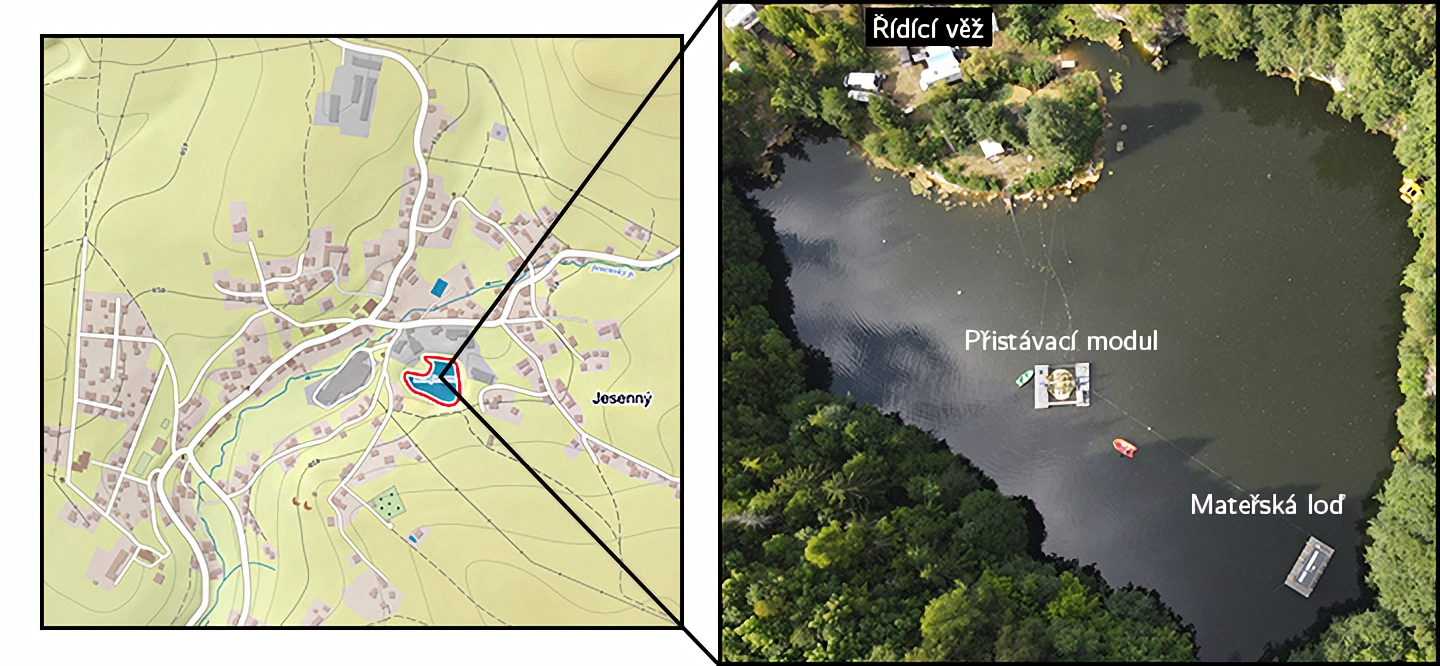
\includegraphics[width=1\linewidth]{figures/map}
        \caption{Detail a lokalita lomu v obci Jesenný (zdroj mapového podkladu: Mapy.cz))}
        \label{fig:map}
    \end{center}
\end{figure}

\subsection{Hlubinná laboratoř H03 DeepLab}
\label{subsubsec:h03_deeplab}
Hydronaut H03 DeepLab je jedinečná výzkumná podvodní laboratoř pro výcvik
posádek v izolovaných, omezených a extrémních podmínkách. Stanice byla zřízena
tak, aby umožnila dlouhodobý pobyt tří členů posádky pod vodní hladinou, přičemž
její konstrukce kombinuje kesonový a ponorkový princip. Díky této unikátní
laboratoří bylo tak umožněno vytvořit podmínky pro dlouhodobý výzkum a sledování
vlivu například tlaku, vlhkosti, stresu, umělého osvětlení a izolovaného
prostředí na člověka nebo použité materiály a vybavení. V rámci mise DIANA plní
roli přistávacího modulu.

\begin{figure}[h]
    \begin{center}
        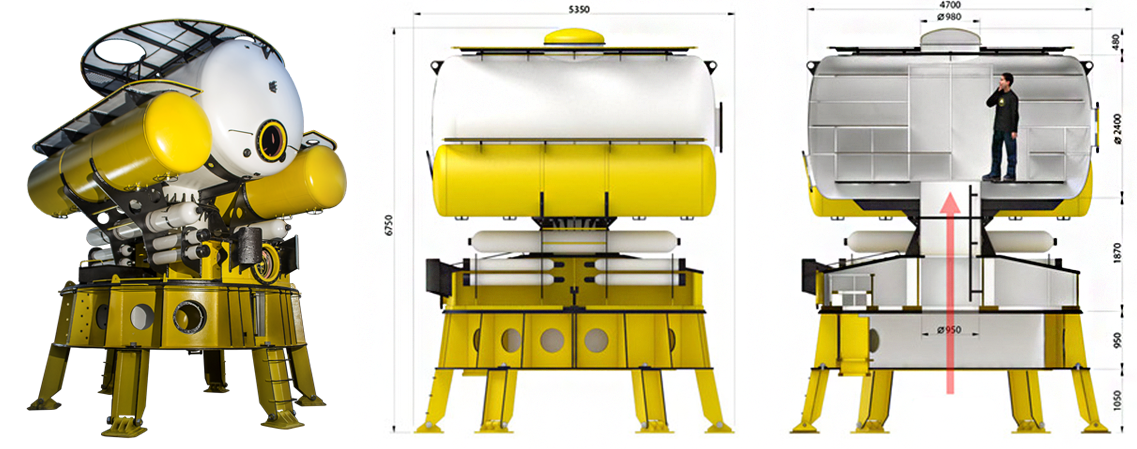
\includegraphics[width=1\linewidth]{figures/habitat}
        \caption{Hlubinná laboratoř H03 DeepLab a její schéma}
        \label{fig:habitat}
    \end{center}
\end{figure}

\subsubsection{Vybavení stanice}
\label{subsubsec:vybaveni_stanice}
Po hardwarové stránce je stanice je vybavena systémy pro monitorování stavu
prostředí uvnitř habitatu a zařízeními pro monitorování fyziologických funkcí
jednotlivých členů posádky. Součástí je také systém pro přenos dat do řídícího
stanoviště. 

Pro potřeby například komunikace nebo monitorování fyziologických dat je stanice
vybavena i potřebným softwarem, který je obalen škálovatelným palubním systémem.
Tento systém umožňuje vizualizaci, administraci a hodnocení měřených veličin
(data prostředí, biomedicínská data) společně s obousměrnou komunikaci se všemi
zapojenými účastníky s možností volby různých komunikačních omezení (např. pro
potřeby simulace výpadku komunikace). Vybrané dílčí částí vybavení stanice jsou
detailněji popsány v následujících sekcích.

\subsubsection{Řízení stanice a mise}
\label{subsubsec:rizeni_stanice_mise}
Stanice H03 DeepLab má hlavní komunikační systém zvaný \textit{Common Tongue}.
Ten zajišťuje komunikaci mezi posádkou a podpůrným týmem a umožňuje živé
sledování životních funkcí posádky a vnitřního prostředí. Pomocí tohoto systému
byli subjektům experimentu zadávány úkoly, které jsou sledovány za účelem
vyhodnocení změn chování sledováním vlivu stresu na soustředění a výkonnost
mozku.

\subsubsection{Monitorování atmosféry habitatu}
Jedním z důležitých východisek pobytu v habitatu jsou podmínky prostředí, které
je nezbytné nepřetržitě a spolehlivě monitorovat. Jednou z těchto podmínek je
atmosféra pro jejiž monitorování slouží systém založený na platformě slowRIO
(slow remote IO controller) vyvinutý ve spolupráci s Fakultou strojní (FS ČVUT)
na projektu Hydronaut. Systém monitoruje a poskytuje data prostředí --
mikroklima: absolutní tlak, relativní vlhkost, teplota vzduchu, teplota vody,
čidlo $O_2$, čidlo $CO_2$, čidlo $H_2$, čidlo $CH_4$, intenzita osvětlení, barva
osvětlení a další. Data jsou posílána do palubního počítače.

\subsection{Infrastruktura mise}
\label{subsec:infrastruktura_mise}
Povaha a náročnost stanovených cílů mise se vyžádaly komplexní infrastrukturu
pro podporu celého výzkumného procesu. V této podsekci je uveden stručný přehled
některých součástí infrastruktury včetně harmonogramu mise. 

\subsubsection{Harmonogram mise}
\label{subsubsec:harmonogram_mise}
Harmonogram mise byl základním dokumentem, který definoval všechny činnosti v
průběhu mise. Harmonogram byl rozepsaný na úroveň minut pro každého jednotlivého
člena posádky. Ukázku harmonogramu lze vidět na Obr.~\ref{fig:harmonogram}. 

\begin{figure}[h]
    \begin{center}
        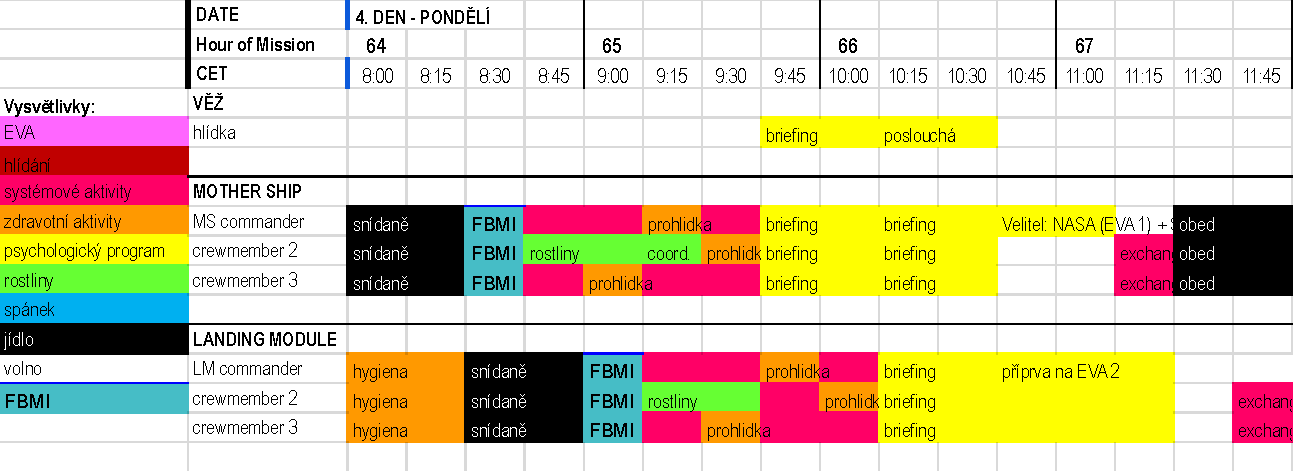
\includegraphics[width=1\linewidth]{figures/harmonogram}
        \caption{Ukázka části harmonogramu mise}
        \label{fig:harmonogram}
    \end{center}
\end{figure}

Spolu s harmonogramem byly vytvořeny další dva dokumenty. První z nich byl plán
směn a druhý byl dokument, do kterého se zaznamenávaly všechny významné
události. Plán směn byl vytvořen interně pro každou instituci, jež byla součástí
mise. Každá směna sloužila primárně za účelem monitorování a dokumentace mise.

\subsubsection{Řídicí věž}
\label{subsubsec:ridici_vez}
Řídicí věž hrála v rámci mise DIANA roli stanoviště na zemi. Komunikovala tedy
se základnou (mateřskou lodí) v souvislosti s prováděním výzkumných a
vzdělávacích programů. Zároveň je zde umístěno monitorovací zařízení posádky,
které nepřetržitě sbírá data a dokumentační a komunikační zařízení. 

\begin{figure}[h]
    \begin{center}
        \includegraphics[width=1\linewidth]{figures/monitoring}
        \caption{Monitorování v řídící věži}
        \label{fig:monitoring}
    \end{center}
\end{figure}

\subsubsection{Povrchová jednotka}
\label{subsubsec:povrchova_jednotka}
Povrchová jednotka byla složena z vedoucího týmu (tři členové stejně jako v
podvodním habitatu), který řídil polohu stanice a systémy podpory života.
Zároveň se povrchová jednotka starala o regulaci specifických parametrů v
závislosti na průběhu mise. Během mise DIANA hrála tato jednotka roli mateřské
lodi, jež sloužila jako stanoviště a kritické zázemí pro velitele posádky. Z
toho místa probíhá ovládání stanice H03 DeepLab. 

\subsubsection{Neuropsychologická baterie}
\label{subsubsec:neuro_testy}
Neuropsychofyziologická stimulace a diagnostika jedinců byla během mise
realizována prostřednictvím:
\begin{enumerate}
    \item \textbf{Kognitivní úlohy v prostředí NEUROP-III} --- posádka opakovaně
    podstoupila náročné diagnostické kognitivní úlohy, zvláště zaměřené na
    sledování exekutivních funkcí primárně v oblasti impulzivního chování,
    riskování, interference nebo inhibice ve smyslu Go-NOGO.
    \item \textbf{Subjektivní hodnocení pomocí NASA TLX} --- jedná se o
    dlouholetý standard pro měření subjektivního vnímání mentální zátěže
    vzhledem ke konkrétním úkolům v pěti dimenzích: mentální náročnost, fyzická
    náročnost, časová náročnost, výkonnost, snaha a frustrace. Posádka byla
    tímto hodnocena během celé mise každý den.
\end{enumerate}

\subsection{Monitorování a měření posádky}
\label{subsec:monitorovani posadky}


\subsubsection{InfluxDB}
\label{subsec:influx}
InfluxDB\footnote{https://www.influxdata.com} je open-source platforma
poskytující databázi pro časové řady. Zahrnuje rozhraní (API) pro standardní
databázové dotazy. Součástí je i grafické uživatelské rozhraní (GUI) s
modulárními uživatelskými panely pro monitorování dat v reálném čase. Tato
platforma (InfluxDB OSS 2.4) byla využita v rámci mise k uchovávání a
vizualizaci dat.

\subsubsection{Měření biosignálů}
\label{subsubsec:mereni_biosignalu}

\subsubsection{Měřící zařízení}
\label{subsubsec:merici_zarizeni}

\subsection{Studie}
\label{subsec:studie}
%!#TODO: Doplnit referenci na prilohu s informovanym souhlasem
Měření dat probíhalo pod Filozofickou fakultou Univerzity Palackého v Olomouci
(\gls{FF UPOL}). Všichni probandi poskytli informované souhlasy pro část
diagnostickou i pro samotný experiment (viz Příloha~\ref{}). Informované
souhlasy umožňují anonymizované využití dat. Získání dat pod FF UPOL probíhalo
podle etického metakodexu Evropské federace psychologických asociací
(\gls{EFPA}). Informované souhlasy jsou i ke všem nahrávkám obrazových dat a
rozhovorů členů posádky. Bezpečí participantů bylo jištěno v několika
technických rovinách prostřednictvím hlavního řešitele \textit{1st Cloud
Republic a.s.} projektu TL05000228.